\documentclass[10pt,a4paper]{article}
\pdfoutput=1
\usepackage[margin=1in,footskip=0.25in]{geometry}

\usepackage{amsmath}
\usepackage{amssymb}
\usepackage{amsthm}
\usepackage{mathtools}
\usepackage{xparse}
\usepackage{cite}
\usepackage{hyperref}
\usepackage{cleveref}
\usepackage{geometry}
\usepackage{pgfplots}
\usepackage{listings}
\usepackage{tikz}
\usepackage{stmaryrd}
\usepackage{float}
\usetikzlibrary{positioning}
\usetikzlibrary{calc}
\usetikzlibrary{quotes}
\usepackage[T1]{fontenc}

\pgfplotsset{compat=1.16}

\newtheorem{claim}{Claim}
\newtheorem{rmk}{Remark}
\newtheorem{defn}[claim]{Definition}
\newtheorem{eg}[claim]{Example}
\newtheorem{lem}[claim]{Lemma}
\newtheorem{thm}[claim]{Theorem}
\newtheorem{cor}[claim]{Corollary}

\DeclareMathOperator{\spn}{span}
\DeclareMathOperator{\diag}{diag}
\DeclareMathOperator{\prj}{Proj}
\DeclareMathOperator{\mat}{Mat}
\DeclareMathOperator{\codim}{codim}

\DeclareMathOperator{\be}{\text{\fontencoding{X2}\selectfont б}}
\DeclareMathOperator{\ve}{\text{\fontencoding{X2}\selectfont в}}
\DeclareMathOperator{\ghe}{\text{\fontencoding{X2}\selectfont г}}

\newcommand{\xrightarrowdbl}[2][]{
  \xrightarrow[#1]{#2}\mathrel{\mkern-14mu}\rightarrow
}

\NewDocumentCommand \bern { O{k} }{
    \rho_{#1}
}

\NewDocumentCommand \calLp { O{n} O{\omega} }{
    {\mathcal L'}^{(#1)}_{#2}
}
\NewDocumentCommand \calL { O{n} O{\alpha^{-n}\omega} }{
    \mathcal L^{(#1)}_{#2}
}
\NewDocumentCommand \Lab { O{a} O{b} }{
    \mathcal L_{#1\rightarrow#2}
}

\newcommand{\ubar}[1]{\text{\b{$#1$}}}

\title{Iterative confusion constraining in imbalanced classification}
\author{George Lee}
\begin{document}
\maketitle
\section{Overview of imbalanced binary classification}
\subsection{Introducton}
Binary classification is a common learning problem:
given an observation in some state space $\mathcal X$, the problem is to construct a model to decide whether $x$ belongs to one of two populations, which we may denote by $+$ and $-$ or by $1$ and $0$.
Of particular interest are cases where $x$ belongs to a majority or a minority class with high and low probability respectively.
When discussing such problems $+$ is typically fixed as the minority class.
In the supervised learning paradigm, models are constructed based on a training set of pairs of inputs and labels $(x,y)\in\mathcal X^m\times\{\pm\}^m$ and subsequently evaluated against a testing set $(a,b)\in\mathcal X^n\times\{\pm\}^n$.

The bulk of popular models use neural networks and we largely focus on this approach here.
One working conjecture is that almost regardless of choice of loss function in such a situation, the gradient updates are likely to fall in a narrow range of possibilities for a fixed batch of training data.
We identify a surface on which we can expect such an update to lie, and propose an algorithm that selects a direction on this surface that forces a particular ratio of false positive and false negatives.
\subsection{Discrete performance metrics for binary classifiers}
When evaluating the model's performance, each binary prediction and label $(\widetilde\upsilon_i,\upsilon_i)$ is either a true positive $(+,+)$, a false positive $(+,-)$, a false negative $(-,+)$ or a true negative $(-,-)$.

When a batch of these observations are made, denote the counts of these corresponding cases by $TP$, $FP$, $FN$ and $TN$ respectively.
Standard associated statistics are
\begin{itemize}
  \item the $\textbf{sample(/batch) precision}=\frac{TP}{TP+FP}$,
  \item the $\textbf{sample recall}=\frac{TP}{TP+FN}$ and
  \item the $\textbf{sample accuracy}=\frac{TP+TN}{TP+FP+TN+FN}$.
\end{itemize}

These quantities are easily understood by someone working on a wide range of possible problems.
In the context of spam filtering, when differentiating between ham and spam, we don't necessarily mind if we sometimes classify ham as spam, but we really should try to insist that spam never makes it through.

You could achieve this by blocking everything, so we can't merely focus on preventing false negatives.
We should try and insist instead on some combination of accuracy and minimising false negatives.

One may also worry about this sort of problem when testing for rare diseases.
Not running any test at all may be highly accurate and possibly preferable to a test with too many false positives.

If we assume that the data is drawn from fixed distributions, then these sample statistics approximate true rates associated to some model with parameter $\boldsymbol\theta$.
Write $\mathbb P_{\boldsymbol\theta}$ for the probabilities of events for such a fixed model.
\begin{itemize}
\item The $\textbf{precision}=\mathbb P_{\boldsymbol\theta}(+|\text{We predicted }+)$, and
\item the $\textbf{recall}=\mathbb P_{\boldsymbol\theta}(\text{we predicted }+|+)$.
\end{itemize}
\subsection{Representing models diagrammatically}
Here 
From the perspective of learning, the function $f_{\boldsymbol\theta}$ defines the inference of a given model with internal state $\boldsymbol\theta$.
This may be represented by the diagram
\begin{figure}[H]
\centering
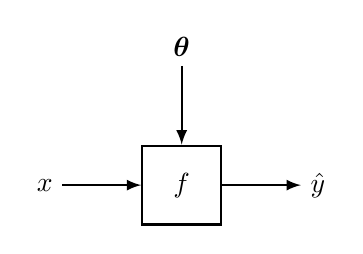
\begin{tikzpicture}
  \node(t) {$\boldsymbol\theta$};
  \node[draw, rectangle, thick, below= of t, minimum height = 1cm,minimum width=1cm] (f) {$f$};
  \node[left= of f] (x) {$x$};
  \node[right= of f] (yh) {$\hat y$};

  \path[-latex, thick, auto] (t) edge (f);
  \path[-latex, thick, auto] (x) edge (f);
  \path[-latex, thick, auto] (f) edge (yh);
\end{tikzpicture}.
\end{figure}
Composition is repredented in an obious way: given another parametric map $g$ whose range is contained in the domain of $f$, the composition $g\fatsemi f$ can be obtained by adding a second block to the left of $f$ which passes its output to $f$.
The composition is then parameterised by the pair $(\theta,\varphi)$.

As well as passing data serially, extra blocks may be added in parallel.
Batching is standard in learning problems, and can be reprented by taking a copy of two blocks that share the same parameterisation.
This may be represented by a a copy operation which is denoted $\Delta$:
\begin{figure}[H]
\centering
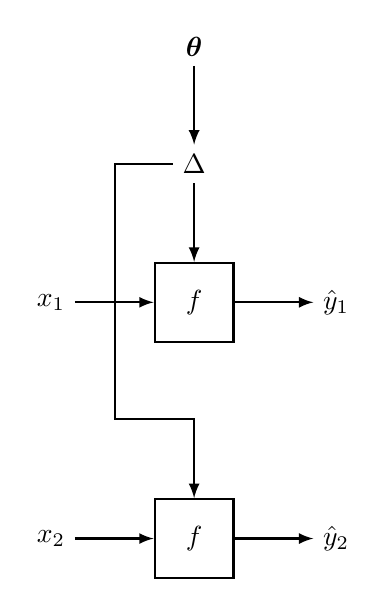
\begin{tikzpicture}
  \node(t) {$\boldsymbol\theta$};
  \node[below=of t](d) {$\Delta$};
  \node[draw, rectangle, thick, below= of d, minimum height = 1cm,minimum width=1cm] (f) {$f$};
  \node[left= of f] (x1) {$x_1$};
  \node[right= of f] (y1) {$\hat y_1$};
  \node[draw, rectangle, thick, minimum height = 1cm,minimum width=1cm] (ff) at ([yshift=-3cm]f) {$f$};
  \node[left= of ff] (x2) {$x_2$};
  \node[right= of ff] (y2) {$\hat y_2$};

  \path[-latex, thick, auto] (t) edge (d);
  \path[-latex, thick, auto] (d) edge (f);
  \path[-latex, thick, auto] (x1) edge (f);
  \path[-latex, thick, auto] (f) edge (y1);

  \path[-latex, thick, auto] (x2) edge (ff);
  \path[-latex, thick, auto] (ff) edge (y2);

  \draw[-latex,thick,auto] (d) to ([xshift=-1cm]d) to ([xshift=-1cm,yshift=1cm]ff.north) to ([yshift=1cm]ff.north)to(ff.north);
\end{tikzpicture}
\\
is a decomposition of\\
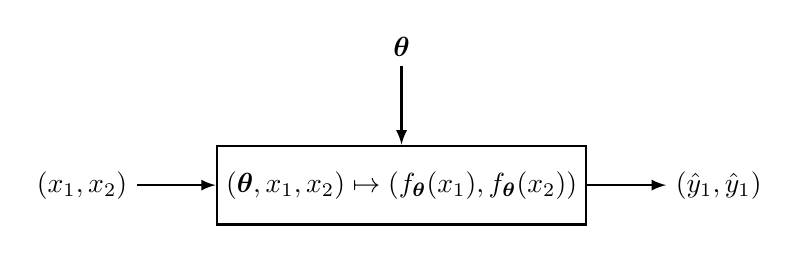
\begin{tikzpicture}
  \node(t) {$\boldsymbol\theta$};
  \node[draw, rectangle, thick, below= of t, minimum height = 1cm,minimum width=1cm] (f) {$(\boldsymbol\theta,x_1,x_2)\mapsto(f_{\boldsymbol\theta}(x_1),f_{\boldsymbol\theta}(x_2))$};
  \node[left= of f] (x) {$(x_1,x_2)$};
  \node[right= of f] (yh) {$(\hat y_1,\hat y_1)$};

  \path[-latex, thick, auto] (t) edge (f);
  \path[-latex, thick, auto] (x) edge (f);
  \path[-latex, thick, auto] (f) edge (yh);
\end{tikzpicture}.
\end{figure}

but there is no way of finding appropriate parameters $\boldsymbol\theta$ without some way of accepting and processing feedback.
In order to better represent the dynamics of algorithms, it is desirable to adopt logically sound notation.
The paper \cite{cruttwell2024deeplearningparametriclenses} is a formal  and a decomposition is sought for the blockIn the diagram above, the parametric function processes data from the left and passes it to the right.
Provided it is sufficiently well behaved, however, such a map can be associated naturally with a backward pass via backpropogation.
Depicted as a single block, each layer within a neural network has incoming and outgoing data to the left, right and its weights above.
There is no requirement in this case for the overall model to pass any data back to the left, and a decomposition is sought for the block
\begin{figure}[H]
\centering
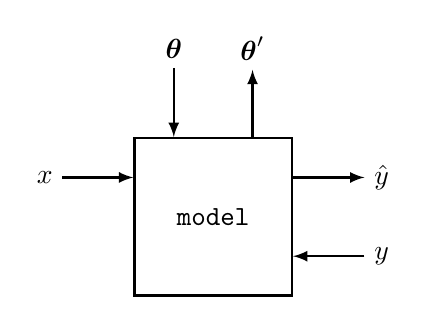
\begin{tikzpicture}
  \node(phi) {$\boldsymbol\theta$};
  \node(t) at ([xshift=.5cm]phi){};
  \node(phip)at ([xshift=.5cm]t) {$\boldsymbol\theta'$};
  \node[draw,below=of t, rectangle, thick, minimum height = 2cm,minimum width=2cm] (f) {$\texttt{model}$};
  \node[left=of f](x){};
  \node(x_in)at([yshift=.5cm]x){$x$};
  \node[right= of f] (y){};
  \node(y_pred) at([yshift=.5cm]y) {$\hat y$};
  \node(y_true)at([yshift=-.5cm]y) {$y$};

  \path[-latex, thick, auto] (phi) edge (f.north -| phi);
  \path[-latex, thick, auto] (f.north -| phip) edge (phip);
  \path[-latex, thick, auto] (x_in) edge (f.west |- x_in);
  \path[-latex, thick, auto] (f.east |- y_pred) edge (y_pred);
  \path[-latex, thick, auto] (y_true) edge (f.east |- y_true);
\end{tikzpicture}
\end{figure}
The map $f$ is referred to as the forward map and $f_\sharp$ is referred to as the backward map.
Each block represents a forced dynamical system.
In these diagrams, the variables above the block represent the internal state of the system.
Arrows flowing in and out of the system are its inputs and outputs respectively.
These diagrams will be developed as particular assumptions are made about $f$ and $f_\sharp$.
In this first example of a lens, the backward map only passes an update up to the internal state of the system.
Correspondingly, as in the next diagram, we also in general allow the backward map to pass values right to left, so that blocks may be composed as coupled dynamical systems that propogate inferences forward and updates backward.
This principle 
\subsection{Thresholded smooth parametric maps}
For any numbers $a,b>0$ the quantity $aFP+bFN$ is analogous to a least squares loss where the cost for a false negative versus a false positive is controlled by $\lambda$.
However, this function takes discrete values so doesn't have a useful gradient and it is impossible to apply backpropogation directly.

The ubiquitous solution here is to work with a model $\tilde f_\theta:\mathcal X\rightarrow(0,1)$ that outputs a number $\tilde f_{\boldsymbol\theta}(x)=\tilde y\in(0,1)$, then take a threshold function $\tau(t)=1$ if $t>\alpha$ and $0$ otherwise for some fixed $\alpha\in(0,1)$ so that
$$
f_{\boldsymbol\theta}(x)=\tau(\tilde f_{\boldsymbol\theta}(x))=\begin{cases*}1~\text{if}~x>\alpha\\
~\text{and}~0~\text{otherwise.}\end{cases*}.
$$
We can represent this diagramatically as a composition of two blocks
\begin{figure}[H]
\centering
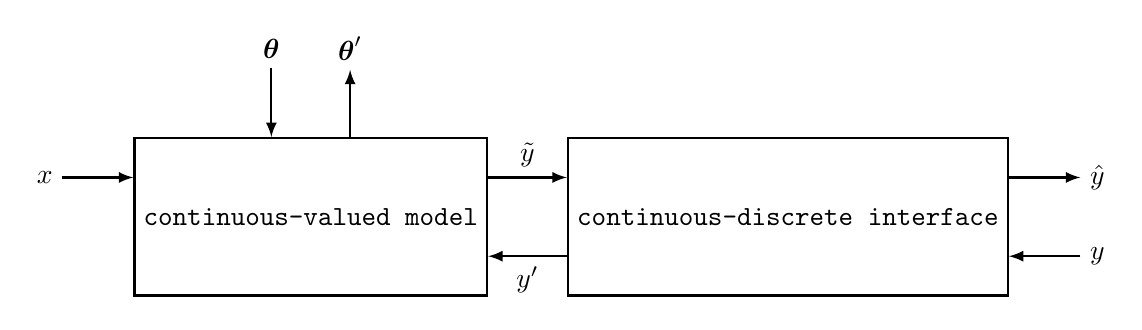
\begin{tikzpicture}
  \node(phi) {$\boldsymbol\theta$};
  \node(t) at ([xshift=.5cm]phi){};
  \node(phip)at ([xshift=.5cm]t) {$\boldsymbol\theta'$};
  \node[draw,below=of t, rectangle, thick, minimum height = 2cm,minimum width=2cm] (f) {$\texttt{continuous-valued model}$};
  \node[draw,right=of f, rectangle, thick, minimum height = 2cm,minimum width=1cm] (thresh) {$\texttt{continuous-discrete interface}$};
  \node[left=of f](x){};
  \node(x_in)at([yshift=.5cm]x){$x$};
  \node[right= of thresh] (y){};
  \node(y_pred) at([yshift=.5cm]y) {$\hat y$};
  \node(y_true)at([yshift=-.5cm]y) {$y$};

  \path[-latex, thick, auto] (phi) edge (f.north -| phi);
  \path[-latex, thick, auto] (f.north -| phip) edge (phip);

  \path[-latex, thick, auto] (x_in) edge (f.west |- x_in);

  \path[-latex, thick, auto] ([yshift=.5cm]f.east) edge["$\tilde y$"] ([yshift=.5cm]thresh.west);
  \path[-latex, thick, auto] ([yshift=-.5cm]thresh.west) edge["$y'$"] ([yshift=-.5cm]f.east);

  \path[-latex, thick, auto] (thresh.east |- y_pred) edge (y_pred);
  \path[-latex, thick, auto] (y_true) edge (thresh.east |- y_true);
\end{tikzpicture}.
\end{figure}
where the forward map of $\texttt{continuous-discrete interface}$ is the thresholding map $\tau$, and the backward map outputs some choice of data encoding the binary performance of the model.
This choice of backward map is nonunique, and in this case a trivial map simply passing back $y$ ould work, but the objective here is to decompose the system into simple components, and this choice simplifies subsequent computation in the backward pass.
The above diagram could be augmented by considering $\alpha$ as a parameter of the model, in which case we would add input threshold $\alpha$ and output $\alpha'$ above the second block to represent its internal state.
$\tau$ and $\tau_\sharp$ would take this extra internal state $\alpha$ as input, and the backward map would output both $z$ and $\alpha'$, $\tau_\sharp(\alpha,\tilde y,y)=(y',\alpha')$, where $\alpha'$ would typically be an updated threshold.
The parameters or internal state of the overall system would then be given by the pair $(\boldsymbol\theta,\alpha)$.
In this work $\alpha=.5$ is fixed, under the assumption that an appropriate choice of $\boldsymbol\theta$ can be found for $\tilde f$ for any threshold that isn't too close to $0$ or $1$.
Indeed, any model which terminates with the single parameter layer $L(\alpha,t)$ taking inputs $t\in(0,1)$ such that
$$
L(\alpha,t)=\begin{cases}\tfrac1{2\alpha}t~\text{if}~t<\tfrac12\text{and}\\\tfrac{t+1-2\alpha}{2(1-\alpha}~\text{otherwise}\end{cases}
$$
demonstrates the redundancy of finding such a threshold as a separate step.
\section{An adaptive gradient rule}

As discussed, it is unfeasible to precisely encode the binary performance of a model using only the gradients of smooth loss functions.
It is nonetheless possible to make a gradient descent type algorithm depend upon such statistics.

\subsection{Smoothed statistics}

Fix a batch of observations $\mathcal F=\{(x_i,y_i)\}_{i=1}^N\subseteq\mathcal X\times\{0,1\}$ and write $\hat y_i=f_{\boldsymbol\theta}(x_i)$ for $1\leq i\leq N$.
As in \cite{lee2021surrogate}, one may  approximate the counts of the four different outcomes algebraically by
\begin{itemize}
  \item $\texttt{tp}_\mathcal F(\boldsymbol\theta)=\sum_{i=1}^N y_i\hat y_i$,
  \item $\texttt{tn}_\mathcal F(\boldsymbol\theta)=\sum_{i=1}^N(1-y_i)(1-\hat y_i)$,
  \item $\texttt{fp}_\mathcal F(\boldsymbol\theta)=\sum_{i=1}^N(1-y_i)\hat y_i$ and
  \item $\texttt{fn}_\mathcal F(\boldsymbol\theta)=\sum_{i=1}^Ny_i(1-\hat y_i)$.
\end{itemize}

Then the estimates for precision and recall are given by
\begin{itemize}
  \item The $\textbf{surrogate precision}=\frac{\texttt{tp}_\mathcal F(\boldsymbol\theta)}{\texttt{tp}_\mathcal F(\boldsymbol\theta)+\texttt{fp}_\mathcal F(\boldsymbol\theta)}$ and
  \item the $\textbf{surrogate recall}=\frac{\texttt{tp}_\mathcal F(\boldsymbol\theta)}{\texttt{tp}_\mathcal F(\boldsymbol\theta)+\texttt{fn}_\mathcal F(\boldsymbol\theta)}$.
\end{itemize}
Where clear we may suppress $\boldsymbol\theta$ and $\mathcal F$ dependence.
Analogously to the binary statistics, writing $|y|=\#\{i:y_i=1\}$ we also have $\texttt{tp}=|y|-\texttt{fn}$ and $\texttt{tn}=|1-y|-\texttt{fp}$.
The values of these quantities are more effort to compute and of little use when evaluating the performance of a model.
Their importance lies in the observation that when used as update functions, the negatives of the gradients of these surrogate false positive and false negative rates tend to force the parameters of the underlying model in the direction of fewer actual false positives and negatives.
If the $\tilde y_i$s were interpreted as probabilities of being in the positive class, then these gradients could be understood as moving the distribution in the direction of maximum likelihood for the batch, but this isn't exactly what the smooth model's target output is.
\subsection{Developing candidate loss functions}
At each point in training, the aim for a classification problem is to update the weights of the smooth model to decrease $\texttt{fn}$ and $\texttt{fp}$ while increasing $\texttt{tn}$ and $\texttt{tp}$.
Write $\partial_{\boldsymbol\theta}$ for derivatives with respect to the parameters.
In choosing a gradient update in these directions, only the smooth false positive and negative gradients need be considered, since $\partial_{\boldsymbol\theta}\texttt{tp}_{\mathcal F}(\boldsymbol\theta)=-\partial_{\boldsymbol\theta}\texttt{fn}_{\mathcal F}(\boldsymbol\theta)$ and $\partial_{\boldsymbol\theta}\texttt{tn}_{\mathcal F}(\boldsymbol\theta)=-\partial_{\boldsymbol\theta}\texttt{fp}_{\mathcal F}(\boldsymbol\theta)$.

The update we generally expect that we will make an update to the parameters in the direction spanned by $\partial_{\boldsymbol\theta}\texttt{tp}_{\mathcal F}(\boldsymbol\theta)$ and $\partial_{\boldsymbol\theta}\texttt{tn}_{\mathcal F}(\boldsymbol\theta)$.
Smooth functions that depend only upon these smooth confusion statistics are essentially the class of ``score oriented loss functions'' described in \cite{marchetti2022score}.
In the case considered here the approach is to allow $U$ and $V$ to depend directly on the discrete performance statistics.
$$
\delta\boldsymbol\theta\propto-U\partial_{\boldsymbol\theta}\texttt{fp}_{\mathcal F}(\boldsymbol\theta)-V\partial_{\boldsymbol\theta}\texttt{fn}_{\mathcal F}(\boldsymbol\theta)=\partial_{\boldsymbol\theta}(-U\texttt{fp}(\boldsymbol\theta)-V\texttt{fn}(\boldsymbol\theta))=\partial_{\boldsymbol\theta}\Phi(\texttt{fp}(\boldsymbol\theta),\texttt{fn}(\boldsymbol\theta),U,V).
$$
Intuitively it might be epected that $U$ and $V>0$ should reflect the relative amount that the model needs to improve on the rates of false positives and false negatives.
Functions similar to $\Phi$, in particular, .
Here the function is allowed to depend upon parameters $U$ and $V$ which can reflect on the actual performance after thresholding.
Correspondingly the overall model may be further decomposed into a network layer followed by a layer which tracks these weights.
In addition, it is often empirically found to be a good idea to not use just the gradient as the update, but typically there is some kind of averaged update, such as adam \cite{kingma2017adammethodstochasticoptimization}.
Introducing a second type of block - a so-called reparameterisation - allows for further factoring of the model into its constituent parts.
The input and output internal state $\boldsymbol\theta=(w,m,c)$ and $\boldsymbol\theta'=(w',m',c')$ is made up of where $(w,w')$ representing the weights of the smooth model, $(m,m')$ the weights of the reparameterisation routine, and $(c,c')$ data dependent upon the binary confusion statistics.
\begin{figure}[H]
\centering
\begin{tikzpicture}
  \node(w) {$w$};
  \node(copy_w) at([yshift=-1.5cm]w) {$\Delta$};
  \node(m)at ([xshift=1cm]w) {$m$};
  \node(tensor_wm)at (m|-copy_w) {$\otimes$};

  \node[draw, rectangle, thick, minimum height = 1cm,minimum width=2cm] (ad)at([xshift=1.5cm,yshift=-3cm]t) {$\texttt{reparameterisation}$};
  \node(wp)at(m-|ad){$w'$};
  \node(mp)at([xshift=1cm]wp){$m'$};
  \node(p_wm)at(wp|-tensor_wm){$\Pi$};

  %\node[below=of ad] (t) {};
  \node(tensor_du) at([yshift=-1cm]ad.south-|wp) {$\otimes$};

  \node[draw, rectangle, thick, minimum height = 2cm,minimum width=2cm] (f) at([yshift=-7cm]t) {$\texttt{smooth}$};
  \node[draw, rectangle, thick, minimum height = 1cm,minimum width=2cm] (fpfn)at([xshift=4cm,yshift=-.5cm]f) {$\texttt{moving averages}$};

  \node[draw,rectangle, thick, minimum height = 2cm,minimum width=1cm] (thresh) at([xshift=8cm]f) {$\texttt{threshold}$};

  \node[left=of f](x){};
  \node(x_in)at([yshift=.5cm]x){$x$};

 \node(D)at([xshift=1cm,yshift=-.5cm]thresh.east){$\Delta$};
  \node[right= of D] (y_true){$y$};
  \node(y_pred) at([yshift=1cm]y_true) {$\hat y$};

  \node(c)at([xshift=-.5cm]fpfn|-w){$c$};
  \node(cp)at([xshift=1cm]c){$c'$};
  \node(p)at(cp|-tensor_du){$\Pi$};

  \path[-latex, thick, auto] (w) edge (copy_w);
  \path[-latex, thick, auto] (m) edge (tensor_wm);
  \path[-latex, thick, auto] (copy_w) edge (tensor_wm);
  \path[-latex, thick, auto] (copy_w) edge (f.north-|copy_w);
  \path[-latex, thick, auto] (tensor_wm) edge (ad.north-|tensor_wm);
  \path[-latex, thick, auto] (ad.north-|p_wm) edge (p_wm);
  \path[-latex, thick, auto] (p_wm)edge(wp);
  \path[thick] (p_wm)edge(p_wm-|mp);
  \path[-latex,thick,auto] (p_wm-|mp)edge(mp);

  \path[thick] (f.north -| m) edge["{$(\partial_w\texttt{fp},\partial_w\texttt{fn})$}",'] (tensor_du -| m);
  \path[-latex,thick,auto] (tensor_du -| m) edge (tensor_du);

  \path[-latex, thick, auto] (tensor_du) edge (ad.south-|tensor_du);

  \path[-latex, thick, auto] (c) edge (fpfn.north -| c);
  \path[-latex, thick, auto] (fpfn.north -| cp) edge (p);
  \path[-latex, thick, auto] (p) edge (cp);
  \path[-latex, thick, auto] (p) edge["{$(U,V)$}",',pos=.6] (tensor_du);

  \path[-latex, thick, auto] (x_in) edge (f.west |- x_in);

  \path[-latex, thick, auto] ([yshift=.5cm]f.east) edge["$\tilde y$",pos=.8] ([yshift=.5cm]thresh.west);
  \path[-latex, thick, auto] (D) edge ([yshift=-.5cm]thresh.east);
  %\path[thick] (D) edge["{$(FP,FN)$}",pos=.7] (junct-|D);
  \draw[-latex,thick,auto] (D) to ([yshift=-1cm]D) to ([xshift=1cm,yshift=-1cm]f.east|-y_true) to ([xshift=1cm]f.east|-y_true)to(f.east|-y_true);

  \path[-latex, thick, auto] (thresh.west|-y_true) edge["{$(FP,FN)$}",'] (fpfn.east|-y_true);


  \path[-latex, thick, auto] (thresh.east |- y_pred) edge (y_pred);
  \path[-latex, thick, auto] (y_true) edge (D);
\end{tikzpicture}
\end{figure}

Correspondingly, we adapt this algorithm to take advantage of the benefits of such an averaging scheme while stll having control over the relative amount that the parameters are updated in favour of false positives or false negatives.
There is freedom to approach the weight updating scheme in many different ways, and we will introduce an explicit choice below.
\lstinputlisting[language=python,basicstyle=\small,caption=A stochastic gradient routineandwith binary prediction derived weighting updates]{snippets/adam_step.py}

\subsection{Comparison with an existing loss function based approach}

In order to control both false positives and false negatives at a specific relative desired rate, one may consider the family of quantities discussed by Rijsbergen in \cite{van1979information}, though here are looking for quantities to minimise so we we modify conventions and use $1-$ the original figure:
$$
F_\beta=1-(1+\beta^2)\frac{\textbf{precision}\cdot\textbf{recall}}{\beta^2\cdot\textbf{precision}+\textbf{recall}}.
$$
This quantity can't be found directly but may be approximated based on a sample, but this won't yield a function to which we can apply gradient descent methods.

swapping out for the surrogates defined above we arrive at what is referred to in \cite{lee2021surrogate} as the macro soft $F_\beta$ score, up to the same modification of convention as before:
\begin{align*}
\texttt F_\beta=&1-(1+\beta^2)\frac{\textbf{surrogate precision}\cdot\textbf{surrogate recall}}{\beta^2\cdot\textbf{surrogate precision}+\textbf{surrogate recall}}\\
=&1-(1+\beta^2)\frac{\texttt{tp}}{\beta^2(\texttt{tp}+\texttt{fn})+\texttt{tp}+\texttt{fp}}\\
  =&\frac{\left(\tfrac{\beta^2}{1+\beta^2}\right)\texttt{fn}+\left(\tfrac1{1+\beta^2}\right)\texttt{fp}}{\texttt{tp}+\left(\tfrac{\beta^2}{1+\beta^2}\right)\texttt{fn}+\left(\tfrac1{1+\beta^2}\right)\texttt{fp}}\\
  =&\frac{\lambda\texttt{fn}+(1-\lambda)\texttt{fp}}{\texttt{tp}+\left(\lambda\texttt{fn}+(1-\lambda)\texttt{fp}\right)}=\frac{\lambda\texttt{fn}+(1-\lambda)\texttt{fp}}{|y|+\left((\lambda-1)\texttt{fn}+(1-\lambda)\texttt{fp}\right)}=\Psi(\texttt{fp},\texttt{fn},\lambda,|y|),
\end{align*}
where $\lambda=\tfrac{\beta^2}{1+\beta^2}$.
One can see from this that the role of $\lambda$ or equivalently $\beta$ is to control the relative cost of a false positive versus a false negative, just as Rijsbergen explains the role of the original $F_\beta$ function in \cite{van1979information}.
Write $\partial_i$ for the partial derivative of a function with respect to its $i$th argument.
The gradient of this loss then is given by
$$
\partial_{\boldsymbol\theta}\texttt{F}_\beta=(\partial_1\Psi)\partial_{\boldsymbol\theta}\texttt{fp}+(\partial_2\Psi)\partial_{\boldsymbol\theta}\texttt{fn}=U_t\partial_{\boldsymbol\theta}\texttt{fp}_t(\boldsymbol\theta_t)+V_t\partial_{\boldsymbol\theta}\texttt{fn}_t(\boldsymbol\theta_t).
$$
If we assume that the performance of a model is already good, so that $|y|\gg\texttt{fp}$ and $\texttt{fn}$, then it is easy to verify that we roughly have
$$
\partial_1\Psi,\partial_2\Psi>0~\text{and}~\frac{\partial_2\Psi}{\partial_1\Psi}\approx\tfrac\lambda{1-\lambda}=\beta^2,
$$
in other words, the relative weighting reflects the target ratio of false positives to false negatives.
This then is an example of a loss that perturbs in a direction in the positive cone spanned by $\partial_{\boldsymbol\theta}\texttt{fp}$ and $\partial_{\boldsymbol\theta}\texttt{fn}$.

Here $U_t$ and $V_t$ are determined by this specific choice of loss - whereas this work makes the relative weighting $U_t$ and $V_t$ more clearly depend on the desired reates of false positives and negatives.

One may also investigate the effect that the relative sizes of $\partial_{\boldsymbol\theta}\texttt{fp}$ and $\partial_{\boldsymbol\theta}\texttt{fn}$: for extreme imbalances it seems likely that this may become important, but empirically this rough argument gives some justification for the choices made in the methods used here.
Note that the use of adam adds some confusion to the analysis by further rescaling the derivatives supplied to it.
\subsection{An adaptive weighting scheme}
Here we give a possible method for choice of weights $U_t$ and $V_t$.
When we are more concerned with reducing false positives, we want $1\approx U_t\gg V_t\approx0$ and vice versa when we are mainly concerned with false negatives.
\lstinputlisting[language=python,basicstyle=\small,caption=Loss weight updating subroutine]{snippets/update_weights.py}
\bibliographystyle{plain}
\bibliography{imbalanced}
\end{document}
